\chapter{Basic formal concepts}\label{chap1}

We introduce formal concepts in Bayesian inference, beginning with Bayes' rule and its components, along with their formal definitions and basic examples. In addition, we present key features of Bayesian inference, such as Bayesian updating and asymptotic sampling properties. We also cover the basics of Bayesian inference from a decision-theoretic perspective under uncertainty, introducing important concepts like loss functions, risk functions, and optimal decision rules.

\section{The Bayes' rule}\label{sec11}
As expected, the starting point for performing Bayesian inference is Bayes' rule,\footnote{Note that I use the term ``Bayes' rule" rather than ``Bayes' theorem." It was Laplace \cite{laplace1774memoire} who generalized Bayes' theorem \cite{bayes1763lii}, and his generalization is referred to as Bayes' rule.} which provides the solution to the inverse problem of determining causes from observed effects. This rule combines prior beliefs with objective probabilities based on repeatable experiments, allowing us to move from observations to probable causes.

Formally, the conditional probability of \( A_i \) given \( B \) is equal to the conditional probability of \( B \) given \( A_i \), multiplied by the marginal probability of \( A_i \), divided by the marginal probability of \( B \),

\begin{align}
	P(A_i\mid B)&=\frac{P(A_i,B)}{P(B)}\nonumber\\
	&=\frac{P(B \mid A_i) \times P(A_i)}{P(B)},
	\label{eq:111}
\end{align}

where, by the law of total probability, \( P(B) = \sum_i P(B \mid A_i) P(A_i) \neq 0 \), and \( \{ A_i, i = 1, 2, \dots \} \) is a finite or countably infinite partition of the sample space.

In the Bayesian framework, \( B \) represents sample information that updates a probabilistic statement about an unknown object \( A_i \) according to probability rules. This is done using Bayes' rule, which incorporates prior ``beliefs" about \( A_i \), i.e., \( P(A_i) \), sample information relating \( B \) to the particular state of nature \( A_i \) through a probabilistic statement, \( P(B \mid A_i) \), and the probability of observing that specific sample information, \( P(B) \).

Let's consider a simple example, \textit{the base rate fallacy}:

Assume that the sample information comes from a positive result from a test whose true positive rate (sensitivity) is 98\%, i.e., \( P(+ \mid \text{disease}) = 0.98 \). On the other hand, the prior information regarding being infected with this disease comes from a base incidence rate of 0.002, i.e., \( P(\text{disease}) = 0.002 \). The question is: \textit{What is the probability of actually being infected, given a positive test result?}

This is an example of \textit{the base rate fallacy}, where a positive test result for a disease with a very low base incidence rate still gives a low probability of actually having the disease.

The key to answering this question lies in understanding the difference between the probability of having the disease given a positive test result, \( P(\text{disease} \mid +) \), and the probability of a positive result given the disease, \( P(+ \mid \text{disease}) \). The former is the crucial result, and Bayes' rule helps us to compute it. Using Bayes' rule (equation \ref{eq:111}):

\begin{align*}
	P(\text{disease}\mid +) & = \frac{P(+\mid \text{disease})\times P(\text{disease})}{P(+)}\\
	& = \frac{0.98 \times 0.002}{0.98 \times 0.002 + (1-0.98) \times (1-0.002)}\\
	& =0.09, 
\end{align*}

where $P(+)=P(+\mid \text{disease})\times P(\text{disease})+P(+\mid \lnot\text{disease})\times P( \lnot\text{disease})$.\footnote{$\lnot$ is the negation symbol. In addition, we have that $P(B\mid A)=1-P(B\mid A^c)$ in this example, where $A^c$ is the complement of $A$. However, it is not always the case that $P(B\mid A)\neq 1-P(B\mid A^c)$.}

The following code shows how to perform this exercise in \textbf{R}.

\begin{tcolorbox}[enhanced,width=4.67in,center upper,
	fontupper=\large\bfseries,drop shadow southwest,sharp corners]
\textit{R code. The base rate fallacy}
\begin{VF}
\begin{lstlisting}[ language=R]
PD <- 0.002 # Probability of disease
PPD <- 0.98 # True positive (Sensitivity)
PDP <- PD * PPD / (PD * PPD + (1 - PD)*(1 - PPD))
paste("Probability of disease given a positive test is", sep = " ", round(PDP, 2))
"Probability of disease given a positive test is 0.09"
\end{lstlisting}
\end{VF}
\end{tcolorbox}

We observe that despite having a positive result, the probability of actually having the disease remains low. This is due to the base rate being so small.

Another interesting example, which lies at the heart of the origin of Bayes' theorem \cite{bayes1763lii}, is related to the existence of God \cite{stigler2018richard}. In Section X of David Hume's ``An Inquiry concerning Human Understanding" (1748), titled \textit{Of Miracles}, Hume argues that when someone claims to have seen a miracle, this provides poor evidence that the event actually occurred, as it contradicts our everyday observations. In response, Richard Price, who finished and published ``An Essay Towards Solving a Problem in the Doctrine of Chances" in 1763 (after Bayes' death in 1761), argues against Hume by highlighting the difference between \textit{impossibility} in casual conversation and \textit{physical impossibility}. Price used an example of a die with a million sides, where \textit{impossibility} refers to rolling a specific side, and \textit{physical impossibility} refers to rolling a side that does not exist. In millions of throws, the latter would never happen, while the former would eventually occur.

Now, let's consider a scenario involving two cases of resurrection (Res): Jesus Christ and Elvis. The total number of people who have ever lived is approximately 108.5 billion,\footnote{\textbf{https://www.wolframalpha.com/input/?i=number+of+people+who+have+ever+lived+on+Earth}} so the prior base rate is given by \( \frac{2}{108.5 \times 10^9} \). On the other hand, suppose the sample information comes from a highly reliable witness with a true positive rate of 0.9999999. The question then is: \textit{What is the probability of this miracle occurring?}.\footnote{\textbf{https://www.r-bloggers.com/2019/04/base-rate-fallacy-or-why-no-one-is-justified-to-believe-that-jesus-rose/}}

Using the Bayes' rule:
{\small{
\begin{align*}
	P(\text{Res}\mid \text{Witness}) & =  \frac{P(\text{Witness}\mid \text{Res})\times P(\text{Res})}{P(\text{Witness})}\\
	& =\frac{2/(108.5 * 10^9) \times 0.9999999}{2/(108.5 * 10^9) \times 0.9999999 + (1-2/(108.5 * 10^9)) \times (1-0.9999999)}\\
	& = 0.000184297806959661
\end{align*}
}}

where $P(\text{Witness})=P(\text{Witness}\mid \text{Res})\times P(\text{Res})+(1-P(\text{Witness}\mid \text{Res}))\times (1-P(\text{Res}))$.

Thus, the probability of a resurrection, given a very reliable witness, is approximately \( 1.843 \times 10^{-4} \).

The following code shows how to perform this exercise in \textbf{R}.

\begin{tcolorbox}[enhanced,width=4.67in,center upper,
	fontupper=\large\bfseries,drop shadow southwest,sharp corners]
\textit{R code. Of Miracles}
\begin{VF}
\begin{lstlisting}[ language=R]
# Probability of resurrection
PR <- 2/(108.5 * 10^9) 
PWR <- 0.9999999 # True positive rate
PRW <- PR * PWR / (PR * PWR + (1 - PR)*(1 - PWR)) 
paste("Probability of resurrection given witness is", sep = " ", PRW)
"Probability of resurrection given witness is 0.000184297806959661"
\end{lstlisting}
\end{VF}
\end{tcolorbox}

Observe that we can condition on multiple events in Bayes' rule. Let's consider two conditioning events, \( B \) and \( C \). Then, equation \ref{eq:111} becomes

\begin{align}
	P(A_i\mid B,C)&=\frac{P(A_i,B,C)}{P(B,C)}\nonumber\\
	&=\frac{P(B\mid A_i,C) \times P(A_i\mid C) \times P(C)}{P(B\mid C)P(C)}.
	\label{eq:112}
\end{align}

Let's use this rule in one of the most intriguing statistical puzzles, \textit{the Monty Hall problem}, to illustrate how to use equation \ref{eq:112} \cite{selvin1975problem,Dawid2016}. This was the situation faced by a contestant in the American television game show \textit{Let's Make a Deal}. In this game, the contestant was asked to choose a door, behind one of which there is a car, and behind the others, goats. 

Let's say the contestant picks door No. 1, and the host (Monty Hall), who knows what is behind each door, opens door No. 3, revealing a goat (see Figure \ref{fig11}). Then, the host asks the tricky question: \textit{Do you want to pick door No. 2?}


\begin{figure}
	
\includegraphics[width=340pt, height=200pt]{Chapters/chapter1/figures/MHproblemNew.png}
	%%\centerline{\epsfig{/Chapters/chapter1/figures/cat.eps,width=.8\textheight,height=.4\textwidth}}
	\caption[List of figure caption goes here]{The Monty Hall show.}\label{fig11}
\end{figure}

Let's define the following events: 

\begin{itemize}
	\item \( P_i \): the event \textbf{contestant picks door No. \( i \)}, which stays closed, 
	\item \( H_i \): the event \textbf{host picks door No. \( i \)}, which is open and contains a goat, 
	\item \( C_i \): the event \textbf{car is behind door No. \( i \)}.
\end{itemize}

In this particular setting, the contestant is interested in the probability of the event \( P(C_2 \mid H_3, P_1) \). A naive answer would be that it is irrelevant, as initially, \( P(C_i) = \frac{1}{3}, \ i = 1, 2, 3 \), and now \( P(C_i \mid H_3) = \frac{1}{2}, \ i = 1, 2 \), since the host opened door No. 3. So, why bother changing the initial guess if the odds are the same (1:1)?

The important point here is that the host knows what is behind each door and always picks a door where there is a goat, given the contestant's choice. In this particular setting:

\[
P(H_3 \mid C_3, P_1) = 0, \quad P(H_3 \mid C_2, P_1) = 1, \quad P(H_3 \mid C_1, P_1) = \frac{1}{2}.
\]

Then, using equation \ref{eq:112}, we can calculate the posterior probability.

\begin{align*}
	P(C_2\mid H_3,P_1)&= \frac{P(C_2,H_3,P_1)}{P(H_3,P_1)}\\
	&= \frac{P(H_3\mid C_2,P_1)P(C_2\mid P_1)P(P_1)}{P(H_3\mid P_1)\times P(P_1)}\\
	&= \frac{P(H_3\mid C_2,P_1)P(C_2)}{P(H_3\mid P_1)}\\
	&=\frac{1\times 1/3}{1/2},
\end{align*}
where the third equation uses the fact that \( C_i \) and \( P_i \) are independent events, and \( P(H_3 \mid P_1) = \frac{1}{2} \) because this depends only on \( P_1 \) (not on \( C_2 \)).

Therefore, changing the initial decision increases the probability of getting the car from \( \frac{1}{3} \) to \( \frac{2}{3} \)! Thus, it is always a good idea to change the door.

Let's see a simulation exercise in \textbf{R} to check this answer:


\begin{tcolorbox}[enhanced,width=4.67in,center upper,
	fontupper=\large\bfseries,drop shadow southwest,sharp corners]
\textit{R code. The Monty Hall problem}
\begin{VF}
\begin{lstlisting}[ language=R]
set.seed(0101) # Set simulation seed
S <- 100000 # Simulations
Game <- function(switch = 0){
	# switch = 0 is not change  
	# switch = 1 is to change
	opts <- 1:3 
	car <- sample(opts, 1) # car location
	guess1 <- sample(opts, 1) # Initial guess 
	
	if(car != guess1) {
	 host <- opts[-c(car, guess1)]
	} else {
	 host <- sample(opts[-c(car, guess1)], 1)
	}	
	win1 <- guess1 == car # Win no change
	guess2 <- opts[-c(host, guess1)]	
	win2 <- guess2 == car # Win change
	if(switch == 0){
		win <- win1
	} else {
		win <- win2
	}
	return(win)
}

#Win probabilities not changing
Prob <- mean(replicate(S, Game(switch = 0))) 
Prob
0.3334

#Win probabilities changing
Prob <- mean(replicate(S, Game(switch = 1))) 
Prob
0.6654
\end{lstlisting}
\end{VF}
\end{tcolorbox}

\section{Bayesian framework: A brief summary of theory}\label{sec12}

Given an unknown parameter set \( \bm{\theta} \), and a particular realization of the data \( \mathbf{y} \), Bayes' rule may be applied analogously,\footnote{From a Bayesian perspective, \( \bm{\theta} \) is fixed but unknown. Then, it is treated as a random object despite the lack of variability (see Chapter \ref{chap2}).}
\begin{align}
	\pi(\bm{\theta}\mid \mathbf{y})&=\frac{p(\mathbf{y}\mid \bm{\theta}) \times \pi(\bm{\theta})}{p(\mathbf{y})},
	\label{eq:121}
\end{align}

where $\pi(\bm{\theta}\mid \mathbf{y})$ is the posterior density function, $\pi(\bm{\theta})$ is the prior density, $p(\mathbf{y}\mid \bm{\theta})$ is the likelihood (statistical model), and

\begin{equation}
	p(\mathbf{y})=\int_{\mathbf{\Theta}}p(\mathbf{y}\mid \bm{\theta})\pi(\bm{\theta})d\bm{\theta}=\mathbb{E}\left[p(\mathbf{y}\mid \bm{\theta})\right]
	\label{eq:121a}
\end{equation}

is the marginal likelihood or prior predictive. Observe that for this expected value to be meaningful, the prior should be a proper density, that is, it must integrate to one; otherwise, it does not make sense.


Observe that \( p(\mathbf{y} \mid \bm{\theta}) \) is not a density in \( \bm{\theta} \). In addition, \( \pi(\bm{\theta}) \) does not have to integrate to 1, that is, \( \pi(\bm{\theta}) \) can be an improper density function, \( \int_{\mathbf{\Theta}} \pi(\bm{\theta}) d\bm{\theta} = \infty \). However, \( \pi(\bm{\theta} \mid \mathbf{y}) \) is a proper density function, that is, \( \int_{\mathbf{\Theta}} \pi(\bm{\theta} \mid \mathbf{y}) d\bm{\theta} = 1 \). 

For instance, set \( \pi(\bm{\theta}) = c \), where \( c \) is a constant, then \( \int_{\mathbf{\Theta}} c d\bm{\theta} = \infty \). However,
\[
\int_{\mathbf{\Theta}} \pi(\bm{\theta} \mid \mathbf{y}) d\bm{\theta} = \int_{\mathbf{\Theta}} \frac{p(\mathbf{y} \mid \bm{\theta}) \times c}{\int_{\mathbf{\Theta}} p(\mathbf{y} \mid \bm{\theta}) \times c \, d\bm{\theta}} d\bm{\theta} = 1
\]
where \( c \) cancels out. 

\(\pi(\bm{\theta} \mid \mathbf{y})\) is a sample updated ``probabilistic belief" version of \(\pi(\bm{\theta})\), where \(\pi(\bm{\theta})\) is a prior probabilistic belief which can be constructed from previous empirical work, theoretical foundations, expert knowledge, and/or mathematical convenience. This prior usually depends on parameters, which are named \textit{hyperparameters}. In addition, the Bayesian approach implies using a probabilistic model about \(\mathbf{Y}\) given \(\bm{\theta}\), that is, \(p(\mathbf{y} \mid \bm{\theta})\), where its integral over \(\mathbf{\Theta}\), \(p(\mathbf{y})\), is named \textit{the model evidence} due to being a measure of model fit to the data.

Observe that the Bayesian inferential approach is conditional, that is, what can we learn about an unknown object \(\bm{\theta}\) given that we already observed \(\bm Y =\mathbf{y}\)? The answer is also conditional on the probabilistic model, that is, \(p(\mathbf{y} \mid \bm{\theta})\). So, what if we want to compare different models, say \(\mathcal{M}_m\), \(m = \{1,2,\dots,M\}\)? Then, we should make explicit this in the Bayes' rule formulation:
\begin{align}
	\pi(\bm{\theta}\mid \mathbf{y},\mathcal{M}_m)&=\frac{p(\mathbf{y}\mid \bm{\theta},\mathcal{M}_m) \times \pi(\bm{\theta}\mid \mathcal{M}_m)}{p(\mathbf{y}\mid \mathcal{M}_m)}.
	\label{eq:122}
\end{align}

The posterior model probability is
\begin{align}
	\pi(\mathcal{M}_m\mid \mathbf{y})&=\frac{p(\mathbf{y}\mid \mathcal{M}_m) \times \pi(\mathcal{M}_m)}{p(\mathbf{y})}, 
	\label{eq:123}
\end{align}

where $p(\mathbf{y}\mid \mathcal{M}_m)=\int_{\mathbf{\Theta}}p(\mathbf{y}\mid \bm{\theta},\mathcal{M}_m) \times \pi(\bm{\theta}\mid \mathcal{M}_m)d\bm{\theta}$ due to equation \ref{eq:122}, and $\pi(\mathcal{M}_m)$ is the prior model probability. 

Calculating \( p(\mathbf{y}) \) in equations \ref{eq:121} and \ref{eq:123} is very demanding in most of the realistic cases. Fortunately, it is not required when performing inference about \( \bm{\theta} \) as this is integrated out from it. Then, all you need to know about the shape of \( \bm{\theta} \) is in \( p(\mathbf{y} \mid \bm{\theta}, \mathcal{M}_m) \times \pi(\bm{\theta} \mid \mathcal{M}_m) \), or without explicitly conditioning on \( \mathcal{M}_m \),
\begin{align}
	\pi(\bm{\theta}\mid \mathbf{y})& \propto p(\mathbf{y}\mid \bm{\theta}) \times \pi(\bm{\theta}).
	\label{eq:124}
\end{align}

Equation \ref{eq:124} is a very good shortcut to perform Bayesian inference about \( \bm{\theta} \).

We can also avoid calculating \( p(\mathbf{y}) \) when performing model selection (hypothesis testing) using the posterior odds ratio, that is, comparing models \( \mathcal{M}_1 \) and \( \mathcal{M}_2 \),

\begin{align}
	PO_{12}&=\frac{\pi(\mathcal{M}_1\mid \mathbf{y})}{\pi(\mathcal{M}_2\mid \mathbf{y})} \nonumber \\
	&=\frac{p(\mathbf{y}\mid \mathcal{M}_1)}{p(\mathbf{y}\mid \mathcal{M}_2)}\times\frac{\pi(\mathcal{M}_1)}{\pi(\mathcal{M}_2)},
	\label{eq:125}
\end{align}

where the first term in equation \ref{eq:125} is named the \textit{Bayes factor}, and the second term is the \textit{prior odds}. Observe that the Bayes factor is a ratio of ordinates for \( \mathbf{y} \) under different models. Then, the Bayes factor is a measure of relative sample evidence in favor of model 1 compared to model 2.

However, we still need to calculate \( p(\mathbf{y}\mid \mathcal{M}_m) = \int_{\mathbf{\Theta}} p(\mathbf{y}\mid \bm{\theta}, \mathcal{M}_m) \pi(\bm{\theta}\mid \mathcal{M}_m) d\bm{\theta} = \mathbb{E}\left[ p(\mathbf{y}\mid \bm{\theta}, \mathcal{M}_m) \right] \). For this integral to be meaningful, the prior must be proper. Using an improper prior has unintended consequences when comparing models; for instance, parsimonious models are favored by posterior odds or Bayes factors, and these values may depend on units of measure (see Chapter \ref{chap4}).

A nice feature of comparing models using posterior odds is that if we have an exhaustive set of competing models such that \( \sum_{m=1}^M \pi(\mathcal{M}_m \mid \mathbf{y}) = 1 \), then we can recover \( \pi(\mathcal{M}_m \mid \mathbf{y}) \) without calculating \( p(\mathbf{y}) \). In particular, given two models \( \mathcal{M}_1 \) and \( \mathcal{M}_2 \) such that \( \pi(\mathcal{M}_1 \mid \mathbf{y}) + \pi(\mathcal{M}_2 \mid \mathbf{y}) = 1 \), we have:
\[
\pi(\mathcal{M}_1 \mid \mathbf{y}) = \frac{PO_{12}}{1 + PO_{12}} \quad \text{and} \quad \pi(\mathcal{M}_2 \mid \mathbf{y}) = 1 - \pi(\mathcal{M}_1 \mid \mathbf{y}).
\]
In general,
\[
\pi(\mathcal{M}_m \mid \mathbf{y}) = \frac{p(\mathbf{y} \mid \mathcal{M}_m) \times \pi(\mathcal{M}_m)}{\sum_{l=1}^M p(\mathbf{y} \mid \mathcal{M}_l) \times \pi(\mathcal{M}_l)}.
\]
These posterior model probabilities can be used to perform Bayesian model averaging.

Table \ref{tab:guide} shows guidelines for the interpretation of \( 2\log(PO_{12}) \) \cite{Kass1995}. This transformation is done to replicate the structure of the likelihood ratio test statistic. However, posterior odds do not require nested models as the likelihood ratio test does.

\begin{table}%1
	%\noautomaticrules
	\tabletitle{Kass and Raftery guidelines.}\label{tab:guide}%
	\begin{tabular}{ccc}
		\textbf{$2\times\log(PO_{12})$}    & \textbf{$PO_{12}$} & \textbf{Evidence against $\mathcal{M}_2$} \\
		\hline
		0 to 2 & 1 to 3 & Not worth more than a bare mention\\
		2 to 6 & 3 to 20 & Positive\\
		6 to 10 & 20 to 150 & Strong\\
		$> 10$  & $> 150$ & Very strong\\
	\end{tabular}
				\begin{tablenotes}[para,flushleft]
	\footnotesize \textit{Notes}: \cite{Kass1995} proposed these guidelines for model selection using posterior odds in a Bayesian framework.\\
\end{tablenotes}
\end{table}
Observe that the posterior odds ratio is a relative criterion, that is, we specify an exhaustive set of competing models and compare them. However, we may want to check the performance of a model on its own or use a non-informative prior. In this case, we can use \textit{the posterior predictive p-value} \cite{Gelman1996,gelman1996posterior}.\footnote{\cite{Bayarri2000} show potential issues due to using data twice in the construction of the predictive p-values. They also present alternative proposals, for instance, \textit{the partial posterior predictive p-value}.}

The intuition behind the predictive p-value is simple: analyze the discrepancy between the model's assumptions and the data by checking a potential extreme tail-area probability. Observe that this approach does not check if a model is true; its focus is on potential discrepancies between the model and the data at hand.

This is done by simulating pseudo-data from our sampling model (\( \mathbf{y}^{(s)}, s=1,2,\dots,S \)) using draws from the posterior distribution, and then calculating a discrepancy measure, \( D(\mathbf{y}^{(s)},\bm{\theta}) \), to estimate the posterior predictive p-value,
\[
p_D(\mathbf{y}) = P[D(\mathbf{y}^{(s)},\bm{\theta}) \geq D(\mathbf{y},\bm{\theta})],
\]
using the proportion of the \( S \) draws for which \( D(\mathbf{y}^{(s)},\bm{\theta}^{(s)}) \geq D(\mathbf{y},\bm{\theta}^{(s)}) \). Extreme tail probabilities (\( p_D(\mathbf{y}) \leq 0.05 \) or \( p_D(\mathbf{y}) \geq 0.95 \)) suggest potential discrepancies between the data and the model. \cite{gelman1996posterior} also suggests the posterior predictive p-value based on the \textit{minimum discrepancy}, 
\[
D_{\min}(\mathbf{y}) = \min_{\bm{\theta}} D(\mathbf{y}, \bm{\theta}),
\]
and the \textit{average discrepancy} statistic 
\[
D(\mathbf{y}) = \mathbb{E}[D(\mathbf{y}, \bm{\theta})] = \int_{\mathbf{\Theta}} D(\mathbf{y}, \bm{\theta}) \pi(\bm{\theta} \mid \mathbf{y}) d\bm{\theta}.
\]
These alternatives can be more computationally demanding.

The Bayesian approach is also suitable to get probabilistic predictions, that is, we can obtain a posterior predictive density 

\begin{align}
	\pi(\mathbf{y}_0\mid \mathbf{y},\mathcal{M}_m) & =\int_{\mathbf{\Theta}}\pi(\mathbf{y}_0,\bm{\theta}\mid \mathbf{y},\mathcal{M}_m)d\bm{\theta}\nonumber\\
	&=\int_{\mathbf{\Theta}}\pi(\mathbf{y}_0\mid \bm{\theta},\mathbf{y},\mathcal{M}_m)\pi(\bm{\theta}\mid \mathbf{y},\mathcal{M}_m)d\bm{\theta}.
	\label{eq:126}
\end{align}

Observe that equation \ref{eq:126} is again an expectation \( \mathbb{E}[\pi(\mathbf{y}_0 \mid \bm{\theta}, \mathbf{y}, \mathcal{M}_m)] \), this time using the posterior distribution. Therefore, the Bayesian approach takes estimation error into account when performing prediction.

As we have shown many times, expectation (integration) is a common feature in Bayesian inference. That is why the remarkable relevance of computation based on \textit{Monte Carlo integration} in the Bayesian framework (see Chapter \ref{chap5}).

\textit{Bayesian model averaging} (BMA) allows for considering model uncertainty in prediction or any unknown probabilistic object. In the case of the predictive density, 

\begin{align}
	\pi(\mathbf{y}_0\mid \mathbf{y})&=\sum_{m=1}^M \pi(\mathcal{M}_m\mid \mathbf{y})\pi(\mathbf{y}_0\mid \mathbf{y},\mathcal{M}_m).
\end{align}
In the case of the posterior density of the parameters,
\begin{align}
	\pi(\bm{\theta}\mid \mathbf{y})&=\sum_{m=1}^M \pi(\mathcal{M}_m\mid \mathbf{y})\pi(\bm{\theta}\mid \mathbf{y},\mathcal{M}_m),
\end{align}
where 
\begin{align}
	\mathbb{E}(\bm{\theta}\mid \mathbf{y})=\sum_{m=1}^{M}\hat{\bm{\theta}}_m \pi(\mathcal{M}_m\mid \mathbf{y}),
	\label{eq:127}
\end{align}
and
\begin{align}
	Var({\theta}_k\mid \mathbf{y})= \sum_{m=1}^{M}\pi(\mathcal{M}_m\mid \mathbf{y}) \widehat{Var} ({\theta}_{km}\mid \mathbf{y},\mathcal{M}_m)+\sum_{m=1}^{M} \pi(\mathcal{M}_m\mid \mathbf{y}) (\hat{{\theta}}_{km}-\mathbb{E}[{\theta}_{km}\mid \mathbf{y}])^2,
	\label{eq:128}
\end{align}
$\hat{\bm{\theta}}_m$ is the posterior mean and $\widehat{Var}({\theta}_{km}\mid \mathbf{y},\mathcal{M}_m)$ is the posterior variance of the $k$-th element of $\bm{\theta}$ under model $\mathcal{M}_m$.

Observe how the variance in equation \ref{eq:128} captures the extra variability due to potential differences between the mean posterior estimates associated with each model, and the posterior mean that incorporates model uncertainty in equation \ref{eq:127}.

A significant advantage of the Bayesian approach, which is particularly useful in \textit{state space representations} (see Chapter \ref{chap8}), is the way the posterior distribution updates with new sample information. Given $\mathbf{y} = \mathbf{y}_{1:t+1}$ as a sequence of observations from 1 to $t+1$, then
\begin{align}\label{equpdate}
	\pi(\bm{\theta}\mid \mathbf{y}_{1:t+1})&\propto p(\mathbf{y}_{1:t+1}\mid \bm{\theta})\times \pi(\bm{\theta})\nonumber\\
	&= p(y_{t+1}\mid \mathbf{y}_{1:t},\bm{\theta})\times p(\mathbf{y}_{1:t}\mid \bm{\theta})\times \pi(\bm{\theta})\nonumber\\
	&\propto p(y_{t+1}\mid \mathbf{y}_{1:t},\bm{\theta})\times \pi(\bm{\theta}\mid \mathbf{y}_{1:t}). 
\end{align}

We observe in Equation \ref{equpdate} that the new prior is simply the posterior distribution based on the previous observations. This is particularly useful under the assumption of \textit{conditional independence}, that is, $Y_{t+1} \perp \mathbf{Y}_{1:t} \mid \bm{\theta}$, so that $p(y_{t+1} \mid \mathbf{y}_{1:t}, \bm{\theta}) = p(y_{t+1} \mid \bm{\theta})$, allowing the posterior to be recovered recursively \cite{petris2009dynamic}. This facilitates online updating because all information up to time $t$ is captured in $\bm{\theta}$. Therefore, $\pi(\bm{\theta} \mid \mathbf{y}_{1:t+1}) \propto p(y_{t+1} \mid \bm{\theta}) \times \pi(\bm{\theta} \mid \mathbf{y}_{1:t}) \propto \prod_{h=1}^{t+1} p(y_h \mid \bm{\theta}) \times \pi(\bm{\theta})$. This recursive expression can be computed more efficiently at any specific point in time $t$, compared to a batch-mode algorithm, which requires processing all information up to time $t$ simultaneously.

It is also important to consider the sampling properties of ``Bayesian estimators". This topic has attracted the attention of statisticians and econometricians for a long time. For instance, asymptotic posterior concentration on the population parameter vector is discussed by \cite{bickel1969some}. The convergence of posterior distributions is stated by the Bernstein-von Mises theorem \cite{Lehmann2003,van2000asymptotic}, which establishes a link between \textit{credible intervals (sets)} and confidence intervals (sets), where a credible interval is an interval in the domain of the posterior distribution within which an unknown parameter falls with a particular probability. Credible intervals treat bounds as fixed and parameters as random, whereas confidence intervals reverse this. There are many settings in parametric models where Bayesian credible intervals with an $\alpha$ level converge asymptotically to confidence intervals at the $\alpha$ level. This suggests that Bayesian inference is asymptotically correct from a sampling perspective in these settings.

A heuristic approach to demonstrate this in the simplest case, where we assume random sampling and $\theta \in \mathcal{R}$, is the following: $p(\mathbf{y} \mid \theta) = \prod_{i=1}^N p(y_i \mid \theta)$, so the log likelihood is $l(\mathbf{y} \mid \theta) \equiv \log p(\mathbf{y} \mid \theta) = \sum_{i=1}^N \log p(y_i \mid \theta) = N \times \bar{l}(\mathbf{y} \mid \theta)$, where $\bar{l} \equiv \frac{1}{N} \sum_{i=1}^N \log p(y_i \mid \theta)$ is the mean likelihood.\footnote{Note that in the likelihood function the argument is $\theta$, but we keep the notation for convenience in exposition.} Then, the posterior distribution is proportional to

\begin{align}
	\pi(\theta\mid \mathbf{y})&\propto p(\mathbf{y}\mid \theta) \times \pi(\theta)\nonumber\\
	&=\exp\left\{N\times \bar{l}(\mathbf{y}\mid \theta)\right\} \times \pi(\theta).
\end{align}

Observe that as the sample size increases, that is, as $N \to \infty$, the exponential term should dominate the prior distribution as long as the prior does not depend on $N$, such that the likelihood determines the posterior distribution asymptotically.

\textit{Maximum likelihood} theory shows that $\lim_{N \to \infty} \bar{l}(\mathbf{y} \mid \theta) \to \bar{l}(\mathbf{y} \mid \theta_0)$, where $\theta_0$ is the population parameter of the data-generating process. In addition, performing a second-order Taylor expansion of the log likelihood at the maximum likelihood estimator,

\begin{align*}
	l(\mathbf{y}\mid \theta)&\approx l(\mathbf{y}\mid \hat{\theta})+\left.\frac{dl(\mathbf{y}\mid {\theta})}{d\theta}\right\vert_{\hat{\theta}}(\theta-\hat{\theta})+\frac{1}{2}\left.\frac{d^2l(\mathbf{y}\mid {\theta})}{d\theta^2}\right\vert_{\hat{\theta}}(\theta-\hat{\theta})^2\\
	&= l(\mathbf{y}\mid \hat{\theta})+\frac{1}{2}\left.\sum_{i=1}^N\frac{d^2l(y_i\mid {\theta})}{d\theta^2}\right\vert_{\hat{\theta}}(\theta-\hat{\theta})^2\\
	&= l(\mathbf{y}\mid \hat{\theta})-\frac{1}{2}\left.N\left[-\bar{l}''\right\vert_{\hat{\theta}}\right](\theta-\hat{\theta})^2\\ 
	&= l(\mathbf{y}\mid \hat{\theta})-\frac{N}{2\sigma^2}(\theta-\hat{\theta})^2 
\end{align*}

where $\left.\frac{dl(\mathbf{y}\mid \theta)}{d\theta}\right\vert_{\hat{\theta}}=0$, $\bar{l}''\equiv\frac{1}{N}\left.\sum_{i=1}^N\frac{d^2l(y_i\mid {\theta})}{d\theta^2}\right\vert_{\hat{\theta}}$ and $\sigma^2:=\left[\left.-\bar{l}''\right\vert_{\hat{\theta}}\right]^{-1}$.\footnote{The last definition follows from standard theory in maximum likelihood estimation (see \cite[Chap. ~10]{casella2024statistical} and \cite[Chap. ~13]{wooldridge2010econometric}).} Then,

\begin{align*}
	\pi(\theta\mid \mathbf{y})&\propto \exp\left\{{l}(\mathbf{y}\mid \theta)\right\} \times \pi(\theta)\\
	&\approx \exp\left\{l(\mathbf{y}\mid \hat{\theta})-\frac{N}{2\sigma^2}(\theta-\hat{\theta})^2\right\} \times \pi(\theta)\\
	&\propto \exp\left\{-\frac{N}{2\sigma^2}(\theta-\hat{\theta})^2\right\} \times \pi(\theta)\\ 
\end{align*}

Observe that the posterior density is proportional to the kernel of a normal density with mean $\hat{\theta}$ and variance $\sigma^2 / N$, as long as $\pi(\hat{\theta}) \neq 0$. This kernel dominates as the sample size increases due to the $N$ in the exponential term. It is also important to note that the prior should not exclude values of $\theta$ that are logically possible, such as $\hat{\theta}$.

\subsection{Example: Health insurance}\label{sec121}
Suppose that you are analyzing whether to buy health insurance next year. To make a better decision, you want to know \textit{what the probability is that you will visit your doctor at least once next year?} To answer this question, you have records of the number of times you have visited your doctor over the last 5 years, \( \mathbf{y} = \{0, 3, 2, 1, 0\} \). How should you proceed?

Assuming that this is a random sample\footnote{Independent and identically distributed draws.} from a data-generating process (statistical model) that is Poisson, i.e., \( Y_i \sim P(\lambda) \), and your probabilistic prior beliefs about \( \lambda \) are well described by a Gamma distribution with shape and scale parameters \( \alpha_0 \) and \( \beta_0 \), i.e., \( \lambda \sim G(\alpha_0, \beta_0) \), then you are interested in calculating the probability \( P(Y_0 > 0 \mid \mathbf{y}) \). To answer this, you need to calculate the posterior predictive density \( \pi(y_0 \mid \mathbf{y}) \) in a Bayesian way.

In this example, \( p(\mathbf{y} \mid \lambda) \) is Poisson, and \( \pi(\lambda) \) is Gamma. Therefore, using Equation \ref{eq:126}.


\begin{align*}
	\pi(y_0\mid \mathbf{y})=&\int_{0}^{\infty}\frac{\lambda^{y_0}\exp\left\{-\lambda\right\}}{y_0!}\times \pi(\lambda\mid \mathbf{y})d\lambda,\\
\end{align*}

where the posterior distribution is $\pi(\lambda\mid \mathbf{y})\propto \lambda^{\sum_{i=1}^N y_i + \alpha_0 - 1}\exp\left\{-\lambda\left(\frac{\beta_0 N+1}{\beta_0}\right)\right\}$ by equation \ref{eq:121}.

Observe that the last expression is the kernel of a Gamma distribution with parameters \( \alpha_n = \sum_{i=1}^N y_i + \alpha_0 \) and \( \beta_n = \frac{\beta_0}{\beta_0 N + 1} \). Given that \( \int_0^{\infty} \pi(\lambda \mid \mathbf{y}) d\lambda = 1 \), the constant of proportionality in the last expression is \( \Gamma(\alpha_n) \beta_n^{\alpha_n} \), where \( \Gamma(\cdot) \) is the Gamma function. Thus, the posterior density function \( \pi(\lambda \mid \mathbf{y}) \) is \( G(\alpha_n, \beta_n) \).

Observe that 
\begin{align*}
	\mathbb{E}[\lambda\mid \mathbf{y}]&=\alpha_n\beta_n\\
	&=\left(\sum_{i=1}^N y_i + \alpha_0\right)\left(\frac{\beta_0}{\beta_0 N + 1}\right)\\
	&=\bar{y}\left(\frac{N\beta_0}{N\beta_0+1}\right)+\alpha_0\beta_0\left(\frac{1}{N\beta_0+1}\right)\\
	&=w\bar{y}+(1-w)\mathbb{E}[\lambda],
\end{align*}

where \( \bar{y} \) is the sample mean estimate, which is the maximum likelihood estimate of \( \lambda \) in this example, \( w = \left(\frac{N\beta_0}{N\beta_0 + 1}\right) \), and \( \mathbb{E}[\lambda] = \alpha_0 \beta_0 \) is the prior mean. The posterior mean is a weighted average of the maximum likelihood estimator (sample information) and the prior mean. Observe that \( \lim_{N \to \infty} w = 1 \), that is, the sample information asymptotically dominates.

The predictive distribution is
\begin{align*}
	\pi(y_0\mid \mathbf{y})=&\int_{0}^{\infty}\frac{\lambda^{y_0}\exp\left\{-\lambda\right\}}{y_0!}\times \frac{1}{\Gamma(\alpha_n)\beta_n^{\alpha_n}}\lambda^{\alpha_n-1}\exp\left\{-\lambda/\beta_n\right\} d\lambda\\
	=&\frac{1}{y_0!\Gamma(\alpha_n)\beta_n^{\alpha_n}}\int_{0}^{\infty}\lambda^{y_0+\alpha_n-1}\exp\left\{-\lambda\left(\frac{1+\beta_n}{\beta_n}\right)\right\}d\lambda\\
	=&\frac{\Gamma(y_0+\alpha_n)\left(\frac{\beta_n}{\beta_n+1}\right)^{y_0+\alpha_n}}{y_0!\Gamma(\alpha_n)\beta_n^{\alpha_n}}\\
	=&{y_0+\alpha_n-1 \choose y_0}\left(\frac{\beta_n}{\beta_n+1}\right)^{y_0}\left(\frac{1}{\beta_n+1}\right)^{\alpha_n}.
\end{align*}

The third equality follows from the kernel of a Gamma density, and the fourth from 
\[
{y_0 + \alpha_n - 1 \choose y_0} = \frac{(y_0 + \alpha_n - 1)(y_0 + \alpha_n - 2)\dots\alpha_n}{y_0!} = \frac{\Gamma(y_0 + \alpha_n)}{\Gamma(\alpha_n) y_0!}
\]
using a property of the Gamma function.

Observe that this is a Negative Binomial density, that is, \( Y_0 \mid \mathbf{y} \sim \text{NB}(\alpha_n, p_n) \) where \( p_n = \frac{\beta_n}{\beta_n + 1} \).

Up to this point, we have said nothing about the hyperparameters, which are required to give a concrete response to this exercise. Thus, we show two approaches to set them. First, we set \( \alpha_0 = 0.001 \) and \( \beta_0 = \frac{1}{0.001} \), which imply vague prior information about \( \lambda \) due to having a large degree of variability compared to the mean information.\footnote{We should be aware that there may be technical problems using this kind of hyperparameters in this setting \cite{gelman2006prior}.} In particular, \( \mathbb{E}[\lambda] = 1 \) and \( \mathbb{V}ar[\lambda] = 1000 \).

In this setting, \( P(Y_0 > 0 \mid \mathbf{y}) = 1 - P(Y_0 = 0 \mid \mathbf{y}) \approx 0.67 \). That is, the probability of visiting the doctor at least once next year is approximately 0.67.

Another approach is using \textit{Empirical Bayes}, where we set the hyperparameters maximizing the logarithm of the marginal likelihood,\footnote{Empirical Bayes methods are criticized due to double-using the data. First to set the hyperparameters, and second, to perform Bayesian inference.} that is,
\[
\left[\hat{\alpha}_0 \ \hat{\beta}_0\right]^{\top} = \underset{\alpha_0, \beta_0}{\mathrm{argmax}} \ \ln p(\mathbf{y})
\]
where
\begin{align*}
	p(\mathbf{y})&=\int_0^{\infty}\left\{\frac{1}{\Gamma(\alpha_0)\beta_0^{\alpha_0}}\lambda^{\alpha_0-1}\exp\left\{-\lambda/\beta_0\right\} \prod_{i=1}^N\frac{\lambda^{y_i}\exp\left\{-\lambda\right\}}{ y_i!}\right\}d\lambda\\
	&=\frac{\int_0^{\infty}\lambda^{\sum_{i=1}^N y_i+\alpha_0-1}\exp\left\{-\lambda \left(\frac{\beta_0 N +1}{\beta_0}\right) \right\}d\lambda}{\Gamma(\alpha_0)\beta_0^{\alpha_0}\prod_{i=1}^N y_i!}\\
	&=\frac{\Gamma(\sum_{i=1}^N y_i+\alpha_0)\left(\frac{\beta_0}{N\beta_0+1}\right)^{\sum_{i=1}^N y_i}\left(\frac{1}{N\beta_0+1}\right)^{\alpha_0}}{\Gamma(\alpha_0)\prod_{i=1}^N y_i}
\end{align*}

Using the empirical Bayes approach, we get $\hat{\alpha}_0 = 51.8$ and $\hat{\beta}_0 = 0.023$, then $P(Y_0 > 0 \mid \mathbf{y}) = 1 - P(Y_0 = 0 \mid \mathbf{y}) \approx 0.70$.

Observe that we can calculate the posterior odds comparing the model using an Empirical Bayes prior (model 1) versus the vague prior (model 2). We assume that $\pi(\mathcal{M}_1) = \pi(\mathcal{M}_2) = 0.5$, then
\begin{align*}
	PO_{12}&=\frac{p(\mathbf{y}\mid \text{Empirical Bayes})}{p(\mathbf{y}\mid \text{Vague prior})}\\
	&=\frac{\frac{\Gamma(\sum_{i=1}^N y_i+51.807)\left(\frac{0.023}{N\times 0.023+1}\right)^{\sum_{i=1}^N y_i}\left(\frac{1}{N\times 0.023+1}\right)^{51.807}}{\Gamma(51.807)}}{\frac{\Gamma(\sum_{i=1}^N y_i+0.001)\left(\frac{1/0.001}{N/0.001+1}\right)^{\sum_{i=1}^N y_i}\left(\frac{1}{N/0.001+1}\right)^{0.001}}{\Gamma(0.001)}}\\
	&\approx 919.
\end{align*}

Then, $2 \times \log(PO_{12}) = 13.64$, which provides very strong evidence against the vague prior model (see Table \ref{tab:guide}). In particular, $\pi(\text{Empirical Bayes} \mid \mathbf{y}) = \frac{919}{1 + 919} = 0.999$ and $\pi(\text{Vague prior} \mid \mathbf{y}) = 1 - 0.999 = 0.001$. These probabilities can be used to perform Bayesian model averaging (BMA). In particular,
\begin{align*}
	\mathbb{E}(\lambda\mid \mathbf{y})&=1.2\times 0.999+1.2\times 0.001=1.2\\
	Var(\lambda\mid \mathbf{y})&=0.025\times 0.999+0.24\times 0.001\\
	& + (1.2-1.2)^2\times 0.999 + (1.2-1.2)^2\times 0.001= 0.025.
\end{align*}

The BMA predictive distribution is a mix of negative binomial distributions, that is, $Y_0\mid \mathbf{y}\sim 0.999\times NB(57.8, 0.02)+0.001\times NB(6.001, 0.17)$.

The following code shows how to perform this exercise in \textbf{R}.

\begin{tcolorbox}[enhanced,width=4.67in,center upper,
	fontupper=\large\bfseries,drop shadow southwest,sharp corners]
\textit{R code. Health insurance, predictive distribution using vague hyperparameters}
\begin{VF}
\begin{lstlisting}[ language=R]
set.seed(010101)
y <- c(0, 3, 2, 1, 0) # Data
N <- length(y)
ProbBo <- function(y, a0, b0){
	N <- length(y)
	#sample size
	an <- a0 + sum(y) 
	# Posterior shape parameter
	bn <- b0 / ((b0 * N) + 1) 
	# Posterior scale parameter
	p <- bn / (bn + 1) 
	# Probability negative binomial density
	Pr <- 1 - pnbinom(0, size=an,prob=(1 - p)) 
	# Probability of visiting the Doctor at least once next year
	# Observe that in R there is a slightly different parametrization.
	return(Pr)
} 
# Using a vague prior:
a0 <- 0.001 # Prior shape parameter
b0 <- 1 / 0.001 # Prior scale parameter
PriMeanV <- a0 * b0 # Prior mean
PriVarV <- a0 * b0^2 # Prior variance
Pp <- ProbBo(y, a0 = 0.001, b0 = 1 / 0.001) 
# This setting is vague prior information.
Pp
0.67
\end{lstlisting}
\end{VF}
\end{tcolorbox} 

\begin{tcolorbox}[enhanced,width=4.67in,center upper,
	fontupper=\large\bfseries,drop shadow southwest,sharp corners]
\textit{R code. Health insurance, predictive distribution using empirical Bayes}
\begin{VF}
\begin{lstlisting}[ language=R]
# Using Empirical Bayes
LogMgLik <- function(theta, y){
 N <- length(y) 
 #sample size
 a0 <- theta[1] 
 # prior shape hyperparameter
 b0 <- theta[2] 
 # prior scale hyperparameter
 an <- sum(y) + a0 
 # posterior shape parameter
 if(a0 <= 0 || b0 <= 0){ 
  #Avoiding negative values
  lnp <- -Inf
  }else{
  lnp <- lgamma(an) + sum(y)*log(b0/(N*b0+1)) - a0*log(N*b0+1) - lgamma(a0)
 } 
 # log marginal likelihood
 return(-lnp)
}			
theta0 <- c(0.01, 1/0.1) 
# Initial values
control <- list(maxit = 1000) 
# Number of iterations in optimization
EmpBay <- optim(theta0, LogMgLik, method = "BFGS", control = control, hessian = TRUE, y = y) 
# Optimization
EmpBay$convergence
0
a0EB <- EmpBay$par[1] 
# Prior shape using empirical Bayes
a0EB
51.81
b0EB <- EmpBay$par[2] 
# Prior scale using empirical Bayes
b0EB
0.023
PriMeanEB <- a0EB * b0EB 
# Prior mean
PriVarEB <- a0EB * b0EB^2 
# Prior variance
PpEB <- ProbBo(y, a0 = a0EB, b0 = b0EB) 
# This setting is using emprical Bayes.
PpEB
0.70 
\end{lstlisting}
\end{VF}
\end{tcolorbox} 

\begin{tcolorbox}[enhanced,width=4.67in,center upper,
	fontupper=\large\bfseries,drop shadow southwest,sharp corners]
	\textit{R code. Health insurance, density plots}
\begin{VF}
\begin{lstlisting}[ language=R]		
# Density figures: 
# This code helps plotting densities
lambda <- seq(0.01, 10, 0.01) 
# Values of lambda
VaguePrior <- dgamma(lambda,shape=a0,scale = b0)
EBPrior <- dgamma(lambda,shape=a0EB,scale = b0EB)
PosteriorV <- dgamma(lambda, shape = a0 + sum(y), scale = b0 / ((b0 * N) + 1)) 
PosteriorEB <- dgamma(lambda, shape = a0EB+sum(y), scale = b0EB / ((b0EB * N) + 1))			
# Likelihood function
Likelihood <- function(theta, y){
 LogL <- dpois(y, theta, log = TRUE)
 Lik <- prod(exp(LogL))
 return(Lik)
}
Liks <- sapply(lambda, function(par) {Likelihood(par, y = y)})
Sc <- max(PosteriorEB)/max(Liks) 
#Scale for displaying in figure
LiksScale <- Liks * Sc
data <- data.frame(cbind(lambda, VaguePrior, EBPrior, PosteriorV, PosteriorEB, LiksScale)) #Data frame
require(ggplot2) # Cool figures
require(latex2exp) # LaTeX equations in figures
require(ggpubr) # Multiple figures in one page
fig1 <- ggplot(data = data, aes(lambda, VaguePrior)) + geom_line() + 	xlab(TeX("$\\lambda$")) + ylab("Density") +	ggtitle("Prior: Vague Gamma") 
fig2 <- ggplot(data = data, aes(lambda, EBPrior)) + geom_line() + xlab(TeX("$\\lambda$")) + ylab("Density") + ggtitle("Prior: Empirical Bayes Gamma")
fig3 <- ggplot(data = data, aes(lambda, PosteriorV)) + geom_line() + xlab(TeX("$\\lambda$")) + ylab("Density") + ggtitle("Posterior: Vague Gamma")
fig4 <- ggplot(data = data, aes(lambda, PosteriorEB)) + geom_line() + xlab(TeX("$\\lambda$")) + ylab("Density") + ggtitle("Posterior: Empirical Bayes Gamma")
FIG <- ggarrange(fig1, fig2, fig3, fig4, ncol = 2, nrow = 2)
annotate_figure(FIG, top = text_grob("Vague versus Empirical Bayes: Poisson-Gamma model", color = "black", face = "bold", size = 14))
dataNew <- data.frame(cbind(rep(lambda, 3), c(EBPrior, PosteriorEB, LiksScale), rep(1:3, each = 1000))) #Data frame
colnames(dataNew) <- c("Lambda", "Density", "Factor")
dataNew$Factor <- factor(dataNew$Factor, levels=c("1", "3", "2"), 
labels=c("Prior", "Likelihood", "Posterior"))
ggplot(data = dataNew, aes_string(x = "Lambda", y = "Density", group = "Factor")) + geom_line(aes(color = Factor)) + xlab(TeX("$\\lambda$")) + ylab("Density") + ggtitle("Prior, likelihood and posterior: Empirical Bayes Poisson-Gamma model") + guides(color=guide_legend(title="Information")) + scale_color_manual(values = c("red", "yellow", "blue"))
\end{lstlisting}
\end{VF}
\end{tcolorbox} 

\begin{figure}[!h]
	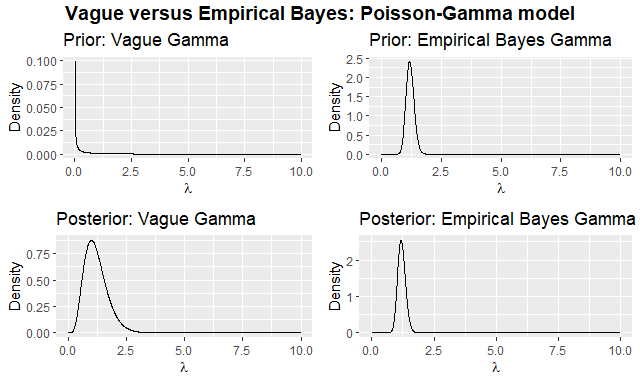
\includegraphics[width=340pt, height=200pt]{Chapters/chapter1/figures/PoisGam.png}
	%%\centerline{\epsfig{/Chapters/chapter1/figures/cat.eps,width=.8\textheight,height=.4\textwidth}}
	\caption[List of figure caption goes here]{Vague versus Empirical Bayes: Poisson-Gamma model.}\label{fig12}
\end{figure}

\begin{figure}[!h]
	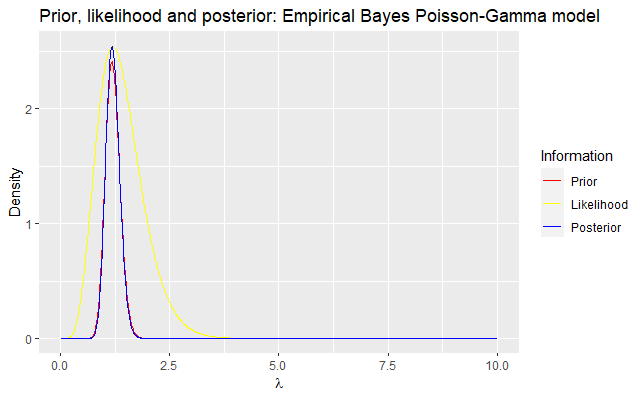
\includegraphics[width=340pt, height=200pt]{Chapters/chapter1/figures/PriorLikPost.png}
	%%\centerline{\epsfig{/Chapters/chapter1/figures/cat.eps,width=.8\textheight,height=.4\textwidth}}
	\caption[List of figure caption goes here]{Prior, likelihood and posterior: Empirical Bayes Poisson-Gamma model.}\label{fig13}
\end{figure}

Figure \ref{fig12} displays the prior and posterior densities based on vague and Empirical Bayes hyperparameters. We observe that the prior and posterior densities using the latter are more informative, as expected.

Figure \ref{fig13} shows the prior, scaled likelihood, and posterior densities of $\lambda$ based on the hyperparameters from the Empirical Bayes approach. The posterior density is a compromise between prior and sample information.

\clearpage
\begin{tcolorbox}[enhanced,width=4.67in,center upper,
	fontupper=\large\bfseries,drop shadow southwest,sharp corners]
\textit{R code. Health insurance, Predictive density}
\begin{VF}
\begin{lstlisting}[
	 language=R]
# Predictive distributions
PredDen <- function(y, y0, a0, b0){
	N <- length(y)
	#sample size
	an <- a0 + sum(y) 
	# Posterior shape parameter
	bn <- b0 / ((b0 * N) + 1) 
	# Posterior scale parameter
	p <- bn / (bn + 1) 
	# Probability negative binomial density
	Pr <- dnbinom(y0, size=an, prob=(1 - p))
	# Predictive density
	# Observe that in R there is a slightly different parametrization.
	return(Pr)
}
y0 <- 0:10
PredVague <- PredDen(y=y, y0=y0, a0=a0, b0=b0)
PredEB <- PredDen(y=y, y0=y0, a0=a0EB, b0=b0EB)
dataPred <- as.data.frame(cbind(y0, PredVague, PredEB))
colnames(dataPred) <- c("y0", "PredictiveVague", "PredictiveEB")
ggplot(data = dataPred) + geom_point(aes(y0, PredictiveVague, color = "red")) +  
xlab(TeX("$y_0$")) + ylab("Density") + ggtitle("Predictive density: Vague and Empirical Bayes priors") + geom_point(aes(y0, PredictiveEB, color = "yellow")) +
guides(color = guide_legend(title="Prior")) + scale_color_manual(labels = c("Vague", "Empirical Bayes"), values = c("red", "yellow")) + scale_x_continuous(breaks=seq(0,10,by=1))
\end{lstlisting}
\end{VF}
\end{tcolorbox}

\begin{figure}[!h]
	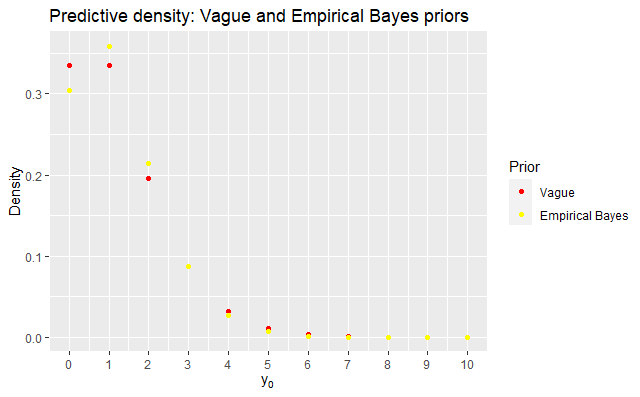
\includegraphics[width=340pt, height=200pt]{Chapters/chapter1/figures/Predictive.png}
	%%\centerline{\epsfig{/Chapters/chapter1/figures/cat.eps,width=.8\textheight,height=.4\textwidth}}
	\caption[List of figure caption goes here]{Predictive density: Vague and Empirical Bayes.}\label{fig14}
\end{figure}

Figure \ref{fig14} displays the predictive probability mass of not having any visits to a physician next year, as well as having one, two, and so on, using Empirical Bayes and vague hyperparameters. The predictive probabilities of not having any visits are approximately 30\% and 33\% based on the Empirical Bayes and vague hyperparameters, respectively.

\begin{tcolorbox}[enhanced,width=4.67in,center upper,
	fontupper=\large\bfseries,drop shadow southwest,sharp corners]
\textit{R code. Health insurance, Bayesian model average}
\begin{VF}
\begin{lstlisting}[language=R]
# Posterior odds: Vague vs Empirical Bayes
PO12 <- exp(-LogMgLik(c(a0EB, b0EB), y = y))/exp(-LogMgLik(c(a0, b0), y = y))
PO12
919
PostProMEM <- PO12/(1 + PO12) 
PostProMEM
0.998
# Posterior model probability Empirical Bayes
PostProbMV <- 1 - PostProMEM 
PostProbMV
0.002
# Posterior model probability vague prior
# Bayesian model average (BMA)
PostMeanEB <- (a0EB + sum(y)) * (b0EB / (b0EB * N + 1)) 
# Posterior mean Empirical Bayes 
PostMeanV <- (a0 + sum(y)) * (b0 / (b0 * N + 1)) 
# Posterior mean vague priors
BMAmean <- PostProMEM * PostMeanEB + PostProbMV * PostMeanV  
BMAmean
1.2
# BMA posterior mean
PostVarEB <- (a0EB + sum(y)) * (b0EB/(b0EB * N + 1))^2 
# Posterior variance Empirical Bayes
PostVarV <- (a0 + sum(y)) * (b0 / (b0 * N + 1))^2 
# Posterior variance vague prior 
BMAVar <- PostProMEM * PostVarEB + PostProbMV*PostVarV + PostProMEM * (PostMeanEB - BMAmean)^2 + PostProbMV * (PostMeanV - BMAmean)^2
# BMA posterior variance   
BMAVar
0.025    
\end{lstlisting}
\end{VF}
\end{tcolorbox}

\begin{tcolorbox}[enhanced,width=4.67in,center upper,
	fontupper=\large\bfseries,drop shadow southwest,sharp corners]
	\textit{R code. Health insurance, Bayesian model average}
	\begin{VF}
		\begin{lstlisting}[ language=R]
# BMA: Predictive
BMAPred <- PostProMEM * PredEB+PostProbMV * PredVague
dataPredBMA <- as.data.frame(cbind(y0, BMAPred))
colnames(dataPredBMA) <- c("y0", "PredictiveBMA")
ggplot(data = dataPredBMA) + geom_point(aes(y0, PredictiveBMA, color = "red")) +  xlab(TeX("$y_0$")) + ylab("Density") + ggtitle("Predictive density: BMA") + guides(color = guide_legend(title="BMA")) + scale_color_manual(labels = c("Probability"), values = c("red")) + scale_x_continuous(breaks=seq(0,10,by=1)) 
		\end{lstlisting}
	\end{VF}
\end{tcolorbox}

\begin{figure}[!h]
	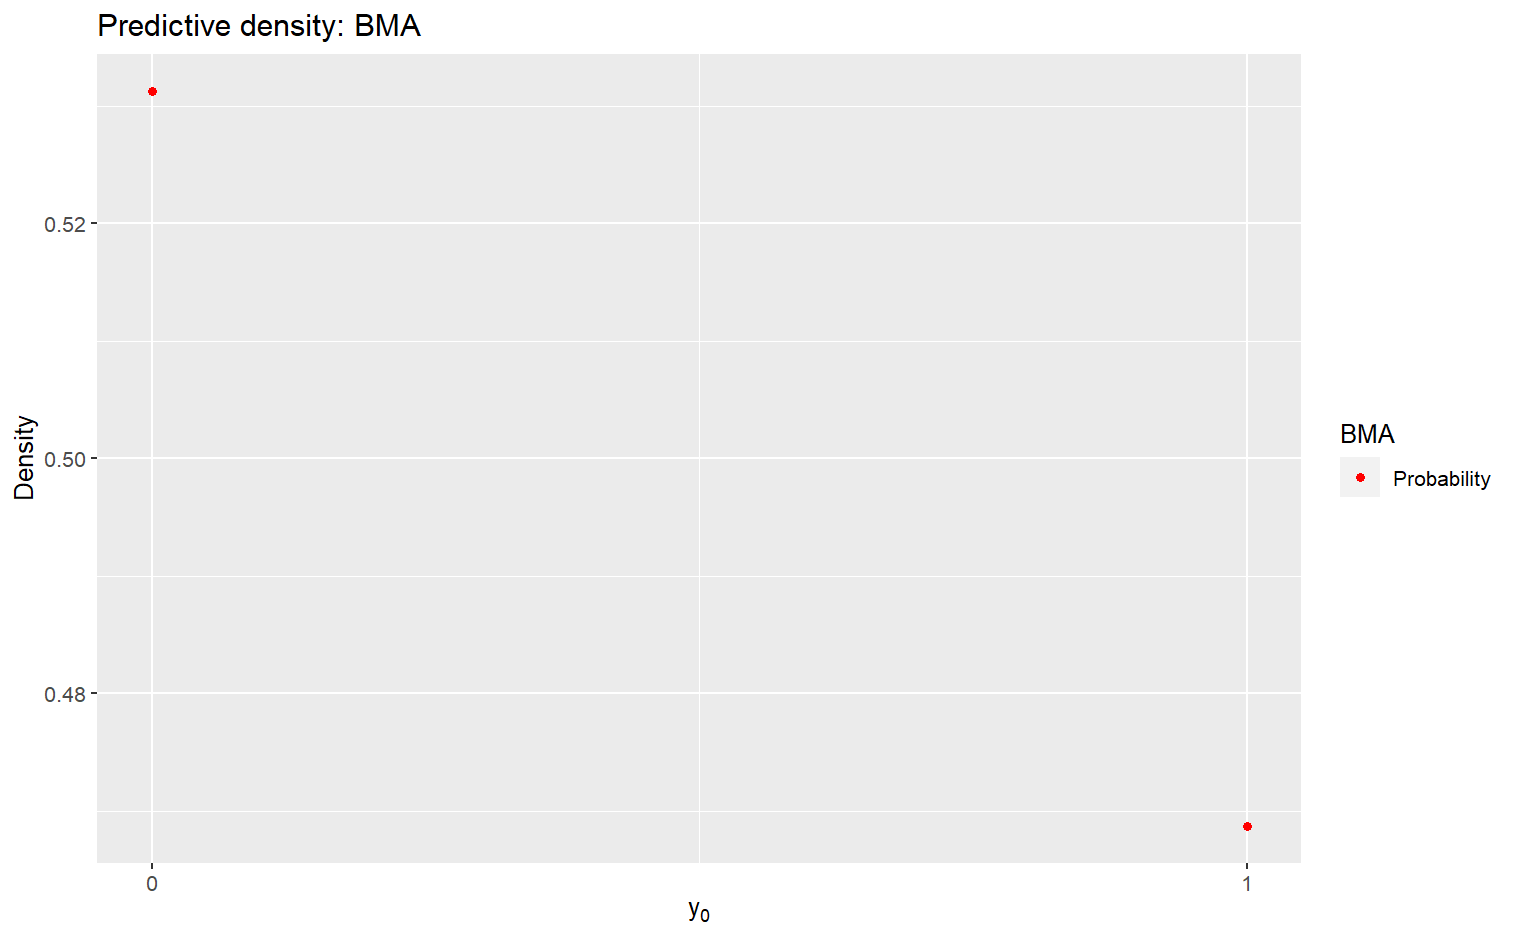
\includegraphics[width=340pt, height=200pt]{Chapters/chapter1/figures/BMA.png}
	%%\centerline{\epsfig{/Chapters/chapter1/figures/cat.eps,width=.8\textheight,height=.4\textwidth}}
	\caption[List of figure caption goes here]{Bayesian model average: Predictive density.}\label{fig15}
\end{figure}

\begin{figure}[!h]
	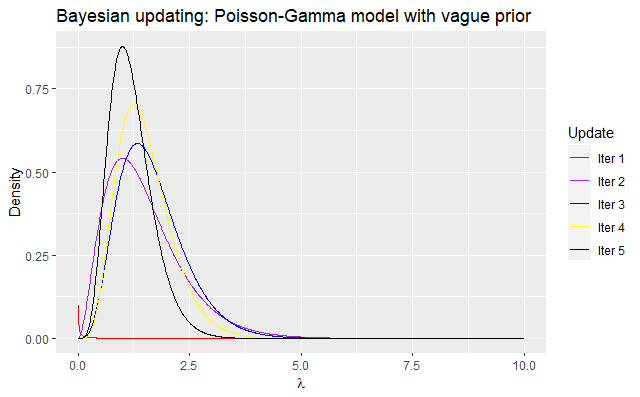
\includegraphics[width=340pt, height=200pt]{Chapters/chapter1/figures/Updating.png}
	%%\centerline{\epsfig{/Chapters/chapter1/figures/cat.eps,width=.8\textheight,height=.4\textwidth}}
	\caption[List of figure caption goes here]{Bayesian updating: Posterior densities.}\label{fig16}
\end{figure}

Figure \ref{fig15} displays the predictive density using Bayesian model averaging based on the vague and Empirical Bayes hyperparameters. This figure closely resembles the predictive probability mass function based on the Empirical Bayes framework, as the posterior model probability for that setting is nearly one.

Figure \ref{fig16} shows how the posterior distribution updates with new sample information, starting from an initial non-informative prior (iteration 1). We observe that iteration 5 incorporates all the sample information in our example. As a result, the posterior density in iteration 5 is identical to the posterior density shown in Figure \ref{fig13}.

\begin{tcolorbox}[enhanced,width=4.67in,center upper,
	fontupper=\large\bfseries,drop shadow southwest,sharp corners]
\textit{R code. Health insurance, Bayes updating}
\begin{VF}
\begin{lstlisting}[ language=R]
# Bayesian updating
BayUp <- function(y, lambda, a0, b0){
	N <- length(y)
	#sample size
	an <- a0 + sum(y) 
	# Posterior shape parameter
	bn <- b0 / ((b0 * N) + 1) 
	# Posterior scale parameter
	p <- dgamma(lambda, shape = an, scale = bn) 
	# Posterior density
	return(list(Post = p, a0New = an, b0New = bn))
}
PostUp <- NULL
for(i in 1:N){
	if(i == 1){
		PostUpi <- BayUp(y[i], lambda, a0 = 0.001, b0 = 1/0.001)}
	else{
		PostUpi <- BayUp(y[i], lambda, a0 = PostUpi$a0New, b0 = PostUpi$b0New)
	}
	PostUp <- cbind(PostUp, PostUpi$Post)
}
DataUp <- data.frame(cbind(rep(lambda, 5), c(PostUp), rep(1:5, each = 1000))) #Data frame
colnames(DataUp) <- c("Lambda", "Density", "Factor")
DataUp$Factor <- factor(DataUp$Factor, levels=c("1", "2", "3", "4", "5"), 
labels=c("Iter 1", "Iter 2", "Iter 3", "Iter 4", "Iter 5"))
ggplot(data = DataUp, aes_string(x = "Lambda", y = "Density", group = "Factor")) + geom_line(aes(color = Factor)) + xlab(TeX("$\\lambda$")) + ylab("Density") + ggtitle("Bayesian updating: Poisson-Gamma model with vague prior") + guides(color=guide_legend(title="Update")) + scale_color_manual(values = c("red", "purple", "blue", "yellow", "black"))
S <- 100000 # Posterior draws
PostMeanLambdaUps <- sapply(1:N, function(i) {mean(sample(lambda, S, replace = TRUE, prob = PostUp[ , i]))}) #Posterior mean update i
paste("Posterior means using all information and sequential updating are:", round(PostMeanV, 2), "and", round(PostMeanLambdaUps[5], 2), sep = " ")
Posterior means using all information and sequential updating are: 1.2 and 1.2 
PostVarLambdaUps <- sapply(1:N, function(i) {var(sample(lambda, S, replace = TRUE, prob = PostUp[ , i]))}) #Posterior variance update i
paste("Posterior variances using all information and sequential updating are:", round(PostVarV, 2), "and", round(PostVarLambdaUps[5], 2), sep = " ")
Posterior variances using all information and sequential updating are: 0.24 and 0.24
\end{lstlisting}
\end{VF}
\end{tcolorbox}

\section{Bayesian reports: Decision theory under uncertainty}\label{sec14}

The Bayesian framework allows reporting the full posterior distributions. However, some situations require reporting a specific value of the posterior distribution (point estimate), an informative interval (set), point or interval predictions, and/or selecting a specific model. Decision theory offers an elegant framework to make decisions regarding the optimal posterior values to report \cite{berger2013statistical}.

The starting point is a \textit{loss function}, which is a non-negative real-valued function whose arguments are the unknown \textit{state of nature} ($\mathbf{\Theta}$), and a set of \textit{actions} to be taken ($\mathcal{A}$), that is, 
\begin{equation*}
	L(\bm{\theta}, a):\mathbf{\Theta}\times \mathcal{A}\rightarrow \mathcal{R}^+.
\end{equation*}

This function is a mathematical representation of the loss incurred from making mistakes. In particular, selecting action $a\in\mathcal{A}$ when $\bm{\theta}\in\mathbf{\Theta}$ is the true state. In our case, the unknown state of nature can refer to parameters, functions of them, future or unknown realizations, models, etc.

From a Bayesian perspective, we should choose the action that minimizes the posterior expected loss ($a^*(\mathbf{y})$), that is, the \textit{posterior risk function} ($\mathbb{E}[L(\bm{\theta}, a)\mid \mathbf{y}]$),
\begin{equation*}
	a^*(\mathbf{y})=\underset{a \in \mathcal{A}}{\mathrm{argmin}} \  \mathbb{E}[L(\bm{\theta}, a)\mid \mathbf{y}], 
\end{equation*}
where $\mathbb{E}[L(\bm{\theta}, a)\mid \mathbf{y}] = \int_{\mathbf{\Theta}} L(\bm{\theta}, a)\pi(\bm{\theta}\mid \mathbf{y})d\bm{\theta}$.\footnote{\cite{Chernozhukov2003} propose Laplace-type estimators (LTE) based on the \textit{quasi-posterior}, $p(\bm{\theta})=\frac{\exp\left\{L_n(\bm{\theta})\right\}\pi(\bm{\theta})}{\int_{\mathbf{\Theta}}\exp\left\{L_n(\bm{\theta})\right\}\pi(\bm{\theta})d\theta}$, where $L_n(\bm{\theta})$ is not necessarily a log-likelihood function. The LTE minimizes the \textit{quasi-posterior risk}.}

Different loss functions imply different optimal decisions. We illustrate this assuming $\theta \in \mathcal{R}$.

\begin{itemize}
	\item The quadratic loss function, $L({\theta},a)=[{\theta}-a]^2$, gives as the optimal decision the posterior mean, $a^*(\mathbf{y})=\mathbb{E}[{\theta}\mid \mathbf{y}]$, that is:
	
	\begin{equation*}
		\mathbb{E}[{\theta}\mid \mathbf{y}] = \underset{a \in \mathcal{A}}{\mathrm{argmin}} \  \int_{{\Theta}} [{\theta}-a]^2\pi({\theta}\mid \mathbf{y})d{\theta}.
	\end{equation*}
	
	To obtain this result, let's use the first-order condition, differentiate the risk function with respect to $a$, interchange the differential and integral order, and set the result equal to zero:
	
	\[
	-2\int_{{\Theta}} [{\theta}-a^*]\pi({\theta}\mid \mathbf{y})d{\theta}=0.
	\]
	
	This implies that
	\[
	a^*\int_{{\Theta}} \pi({\theta}\mid \mathbf{y})d{\theta}=a^*(\mathbf{y})=\int_{{\Theta}} {\theta}\pi({\theta}\mid \mathbf{y})d{\theta}=\mathbb{E}[{\theta}\mid \mathbf{y}],
	\]
	that is, the posterior mean is the Bayesian optimal action. This means that we should report the posterior mean as a point estimate of $\theta$ when facing the quadratic loss function.
	
	\item The generalized quadratic loss function, $L({\theta},a)=w({\theta})[{\theta}-a]^2$, where $w({\theta})>0$ is a weighting function, gives as the optimal decision rule the weighted mean. We should follow the same steps as the previous result to obtain
	\[
	a^*(\mathbf{y})=\frac{\mathbb{E}[w({\theta})\times{\theta}\mid \mathbf{y}]}{\mathbb{E}[w({\theta})\mid \mathbf{y}]}.
	\]
	Observe that the weighted average is driven by the weighting function $w({\theta})$.
	
	\item The absolute error loss function, $L({\theta},a)=|{\theta}-a|$, gives as the optimal action the posterior median (Exercise 5).
	
	\item The generalized absolute error function,
	
	\begin{equation*}
		L(\theta,a)=\begin{cases} 
			K_0(\theta-a), & \theta-a \geq 0, \\
			K_1(a-\theta), & \theta-a < 0, 
		\end{cases} \quad K_0, K_1 > 0,
	\end{equation*}
	
	implies the following risk function:
	
	\begin{align*}
		\mathbb{E}[L(\theta, a)\mid \mathbf{y}] &= \int_{-\infty}^a K_1(a-\theta)\pi(\theta\mid \mathbf{y})d\theta + \int_a^{\infty} K_0(\theta-a)\pi(\theta\mid \mathbf{y})d\theta. 
	\end{align*}
	
	Differentiating with respect to $a$, interchanging differentials and integrals, and equating to zero, we get:
	
	\begin{align*}
		K_1\int_{-\infty}^{a^*} \pi(\theta\mid \mathbf{y})d\theta - K_0\int_{a^*}^{\infty} \pi(\theta\mid \mathbf{y})d\theta &= 0.
	\end{align*}
	
	Thus, we have
	\[
	\int_{-\infty}^{a^*} \pi(\theta\mid \mathbf{y})d\theta = \frac{K_0}{K_0 + K_1},
	\]
	that is, any $\frac{K_0}{K_0 + K_1}$-percentile of $\pi(\theta\mid \mathbf{y})$ is an optimal Bayesian estimate of $\theta$.
\end{itemize}

We can also use decision theory under uncertainty in hypothesis testing. In particular, testing $H_0:\theta\in\Theta_0$ versus $H_1:\theta\in\Theta_1$, where $\Theta=\Theta_0 \cup \Theta_1$ and $\emptyset=\Theta_0 \cap \Theta_1$, there are two actions of interest, $a_0$ and $a_1$, where $a_j$ denotes not rejecting $H_j$, for $j=\{0,1\}$.

Given the $0-K_j$ loss function:

\begin{equation*}
	L(\theta,a_j)=\begin{cases} 
		0, & \text{if } \theta \in \Theta_j, \\
		K_j, & \text{if } \theta \in \Theta_i, j \neq i,
	\end{cases}
\end{equation*}

where there is no loss if the right decision is made, for instance, not rejecting $H_0$ when $\theta \in \Theta_0$, and the loss is $K_j$ when an error is made. For example, a type I error occurs when rejecting the null hypothesis ($H_0$) when it is true ($\theta \in \Theta_0$), which results in a loss of $K_1$ due to choosing action $a_1$, not rejecting $H_1$.

The posterior expected loss associated with decision $a_j$, i.e., not rejecting $H_j$, is:
\[
\mathbb{E}[L(\theta,a_j) \mid \mathbf{y}] = 0 \times P(\Theta_j \mid \mathbf{y}) + K_j P(\Theta_i \mid \mathbf{y}) = K_j P(\Theta_i \mid \mathbf{y}), \quad j \neq i.
\]

Therefore, the Bayes optimal decision is the one that minimizes the posterior expected loss. That is, the null hypothesis is rejected ($a_1$ is not rejected) when
\[
K_0 P(\Theta_1 \mid \mathbf{y}) > K_1 P(\Theta_0 \mid \mathbf{y}).
\]

Given our framework, $\Theta = \Theta_0 \cup \Theta_1$ and $\emptyset = \Theta_0 \cap \Theta_1$, we have $P(\Theta_0 \mid \mathbf{y}) = 1 - P(\Theta_1 \mid \mathbf{y})$. As a result, the rejection region of the Bayesian test is:
\[
R = \left\{ \mathbf{y}: P(\Theta_1 \mid \mathbf{y}) > \frac{K_1}{K_1 + K_0} \right\}.
\]

Decision theory also helps to construct interval (region) estimates. Let $\Theta_{C(\mathbf{y})} \subset \Theta$ be a \textit{credible set} for $\theta$, and let the loss function be defined as:
\[
L(\theta, \Theta_{C(\mathbf{y})}) = 1 - \mathbbm{1}\left\{\theta \in \Theta_{C(\mathbf{y})}\right\},
\]
where
\[
\mathbbm{1}\left\{\theta \in \Theta_{C(\mathbf{y})}\right\} = \begin{cases} 
	1, & \text{if } \theta \in \Theta_{C(\mathbf{y})}, \\
	0, & \text{if } \theta \notin \Theta_{C(\mathbf{y})}.
\end{cases}
\]

Thus, the loss function becomes:
\[
L(\theta, \Theta_{C(\mathbf{y})}) = \begin{cases} 
	0, & \text{if } \theta \in \Theta_{C(\mathbf{y})}, \\
	1, & \text{if } \theta \notin \Theta_{C(\mathbf{y})}.
\end{cases}
\]

This is a 0--1 loss function, which equals zero when $\theta \in \Theta_{C(\mathbf{y})}$ and equals one when $\theta \notin \Theta_{C(\mathbf{y})}$. Consequently, the risk function is:
\[
1 - P(\theta \in \Theta_{C(\mathbf{y})}).
\]

Given a \textit{measure of credibility} $\alpha(\mathbf{y})$ that defines the level of trust that $\theta \in \Theta_{C(\mathbf{y})}$, we can measure the accuracy of the report by the loss function:
\[
L(\theta, \alpha(\mathbf{y})) = \left[\mathbbm{1}\left\{\theta \in \Theta_{C(\mathbf{y})}\right\} - \alpha(\mathbf{y})\right]^2.
\]

This loss function could be used to suggest a choice of the report $\alpha(\mathbf{y})$. Given that this is a quadratic loss function, the optimal action is the posterior mean, that is,
\[
\mathbb{E}[\mathbbm{1}\left\{\theta \in \Theta_{C(\mathbf{y})}\right\} \mid \mathbf{y}] = P(\theta \in \Theta_{C(\mathbf{y})} \mid \mathbf{y}).
\]

This probability can be calculated given the posterior distribution as
\[
P(\theta \in \Theta_{C(\mathbf{y})} \mid \mathbf{y}) = \int_{\Theta_{C(\mathbf{y})}} \pi(\theta \mid \mathbf{y}) d\theta.
\]

This represents a measure of the belief that $\theta \in \Theta_{C(\mathbf{y})}$ given the prior beliefs and sample information.

The set $\Theta_{C(\mathbf{y})} \subset \Theta$ is a $100(1-\alpha)\%$ credible set with respect to $\pi(\theta \mid \mathbf{y})$ if
\[
P(\theta \in \Theta_{C(\mathbf{y})} \mid \mathbf{y}) = \int_{\Theta_{C(\mathbf{y})}} \pi(\theta \mid \mathbf{y}) d\theta = 1 - \alpha.
\]

Two alternatives for reporting credible sets are the \textit{symmetric credible set} and the \textit{highest posterior density set} (HPD). The former is based on the $\frac{\alpha}{2}\%$ and $(1 - \frac{\alpha}{2})\%$ percentiles of the posterior distribution, and the latter is a $100(1 - \alpha)\%$ credible interval for $\theta$ with the property that it has the smallest distance compared to any other $100(1 - \alpha)\%$ credible interval for $\theta$ based on the posterior distribution. Specifically,
\[
C(\mathbf{y}) = \left\{ \theta : \pi(\theta \mid \mathbf{y}) \geq k(\alpha) \right\},
\]

where $k(\alpha)$ is the largest number such that
\[
\int_{\theta : \pi(\theta \mid \mathbf{y}) \geq k(\alpha)} \pi(\theta \mid \mathbf{y}) d\theta = 1 - \alpha.
\]

The HPD set can be a collection of disjoint intervals when working with multimodal posterior densities. Additionally, HPD sets have the limitation of not necessarily being invariant under transformations.

Decision theory can also be used to perform prediction (point, sets, or probabilistic). Suppose that there is a loss function $L(Y_0, a)$ involving the prediction of $Y_0$. Then, the expected loss is
\[
\mathbb{E}_{Y_0}[L(Y_0, a)] = \int_{\mathcal{Y}_0} L(y_0, a) \pi(y_0 \mid \mathbf{y}) \, dy_0,
\]

where $\pi(y_0 \mid \mathbf{y})$ is the predictive density function. Thus, we make an optimal choice for prediction that minimizes the risk function given a specific loss function.

Although Bayesian Model Averaging (BMA) allows for incorporating model uncertainty in a regression framework, sometimes it is desirable to select just one model. A compelling alternative is to choose the model with the highest posterior model probability. This model is the best alternative for prediction in the case of a 0-1 loss function \cite{Clyde2004}.

\subsection{Example: Health insurance continues}\label{131}

We show some optimal rules in the health insurance example, specifically the best point estimates of $\lambda$ under the quadratic, absolute, and generalized absolute loss functions. For the generalized absolute loss function, we assume that underestimating $\lambda$ is twice as costly as overestimating it, i.e., $K_0 = 2$ and $K_1 = 1$.

Given that the posterior distribution of $\lambda$ is $G(\alpha_0 + \sum_{i=1}^N y_i, \frac{\beta_0}{\beta_0 N + 1})$, and using the hyperparameters from empirical Bayes, we obtain the following optimal point estimates:
\begin{itemize}
	\item The posterior mean: $\mathbb{E}[\lambda \mid \mathbf{y}] = \alpha_n \beta_n = 1.2$,
	\item The posterior median: 1.19,
	\item The 2/3-th quantile: 1.26.
\end{itemize}
These are the optimal point estimates for the quadratic, absolute, and generalized absolute loss functions, respectively.

In addition, we test the null hypothesis $H_0: \lambda \in [0, 1)$ versus the alternative hypothesis $H_1: \lambda \in [1, \infty)$, setting $K_0 = K_1 = 1$. We should reject the null hypothesis since $P(\lambda \in [0, 1)) = 0.9 > \frac{K_1}{K_0 + K_1} = 0.5$.

The 95\% symmetric credible interval is $(0.91, 1.53)$, and the highest posterior density (HPD) interval is $(0.90, 1.51)$. Finally, the optimal point prediction under the quadratic loss function is 1.2, which is the mean value of the posterior predictive distribution. The optimal model, assuming a 0-1 loss function, is the model using the hyperparameters from the empirical Bayes procedure, since the posterior model probability of this model is approximately 1, whereas the posterior model probability of the model using vague hyperparameters is approximately 0.

\begin{tcolorbox}[enhanced,width=4.67in,center upper,
	fontupper=\large\bfseries,drop shadow southwest,sharp corners]
	\textit{R code. Health insurance, Bayesian reports}
\begin{VF}
\begin{lstlisting}[ language=R]
an <- sum(y) + a0EB 
# Posterior shape parameter
bn <- b0EB / (N*b0EB + 1) 
# Posterior scale parameter
S <- 1000000 
# Number of posterior draws
Draws <- rgamma(1000000, shape = an, scale = bn) 
# Posterior draws
###### Point estimation ########
OptQua <- an*bn 
# Mean: Optimal choice quadratic loss function
OptQua
1.200952
OptAbs <- qgamma(0.5, shape = an, scale = bn) 
# Median: Optimal choice absolute loss function
OptAbs
1.194034
# Setting K0 = 2 and K1 = 1, that is, to underestimate lambda is twice as costly as to overestimate it.
K0 <- 2; K1 <- 1
OptGenAbs <- quantile(Draws, K0/(K0 + K1)) 
# Median: Optimal choice generalized absolute loss function
OptGenAbs
66.66667% 
1.262986 
###### Hypothesis test ########
# H0: lambda in [0,1) vs H1: lambda in [1, Inf]
K0 <- 1; K1 <- 1
ProbH0 <- pgamma(1, shape = an, scale = bn) 
ProbH0 # Posterior  probability H0
0.09569011
ProbH1 <- 1 -ProbH0
ProbH1 # Posterior  probability H1
0.9043099
# We should reject H0 given ProbH1 > K1 / (K0 + K1) 
###### Credible intervals ########
LimInf <- qgamma(0.025, shape = an, scale = bn) # Lower bound
LimInf
0.9114851
LimSup <- qgamma(0.975, shape = an, scale = bn) # Upper bound
LimSup
1.529724
HDI <- HDInterval::hdi(Draws, credMass = 0.95) # Highest posterior density credible interval
HDI
    lower     upper 
0.8971505 1.5125911 
attr(,"credMass")
[1] 0.95
###### Predictive optimal choices ########
p <- bn / (bn + 1) # Probability negative binomial density
OptPred <- p/(1-p)*an # Optimal point prediction given a quadratic loss function in prediction
OptPred
1.200952
\end{lstlisting}
\end{VF}
\end{tcolorbox}

\section{Summary}
We introduce Bayes' rule to update probabilistic statements using humorous examples. We then study the three key probabilistic objects in Bayesian inference: the posterior distribution, the marginal likelihood, and the predictive density. The posterior distribution allows for inference regarding parameters, the marginal likelihood is required for hypothesis testing and model selection using the Bayes factor, and the predictive density enables probabilistic predictions. We also review some sampling properties of Bayesian estimators and the process of Bayes updating. All of these concepts were illustrated using a simple example in \textbf{R} software. Finally, we introduce decision theory concepts that can be applied to report summary statistics while minimizing posterior expected losses.
 
\section{Exercises}

\begin{enumerate}
	\item \textit{The Court Case: The Blue or Green Cab}
	
	A cab was involved in a hit-and-run accident at night. There are two cab companies in the town: Blue and Green. The former has 150 cabs, and the latter has 850 cabs. A witness stated that a blue cab was involved in the accident; the court tested the reliability of the witness under similar circumstances and found that 80\% of the time the witness correctly identified the color of the cab. \textit{What is the probability that the color of the cab involved in the accident was blue, given that the witness said it was blue?}
	
	\item \textit{The Monty Hall Problem}
	
	What is the probability of winning a car in the \textit{Monty Hall problem} if you switch your decision, when there are four doors, three goats, and one car? Solve this problem both analytically and computationally. What if there are $n$ doors, $n-1$ goats, and one car?
	
	\item Solve the health insurance example using a Gamma prior in the rate parametrization, that is, $\pi(\lambda) = \frac{\beta_0^{\alpha_0}}{\Gamma(\alpha_0)} \lambda^{\alpha_0 - 1} \exp\left\{-\lambda \beta_0\right\}$.
	
	\item Suppose you are analyzing the decision to buy car insurance for the next year. To make a better decision, you want to know: \textit{What is the probability that you will have a car claim next year?} You have the records of your car claims over the last 15 years, $\mathbf{y} = \left\{ 0, 1, 0, 1, 0, 1, 1, 0, 0, 1, 0, 0, 1, 1, 0 \right\}$.
	
	Assume that this is a random sample from a data-generating process (statistical model) that is Bernoulli, $Y_i \sim \text{Ber}(p)$. Your prior beliefs about $p$ are well described by a Beta distribution with parameters $\alpha_0$ and $\beta_0$, i.e., $p \sim B(\alpha_0, \beta_0)$. You are interested in calculating the probability of a claim the next year, $P(Y_0 = 1 \mid \mathbf{y})$.
	
	Solve this using both an empirical Bayes approach and a non-informative approach where $\alpha_0 = \beta_0 = 1$ (uniform distribution).
	
	\item Show that, given the loss function $L(\theta, a) = |\theta - a|$, the optimal decision rule minimizing the risk function, $a^*(\mathbf{y})$, is the median.
	
\end{enumerate}



